% Number 180
% CVPMA Algebra Units 
% Problem-solving, RC cars passing each other - hardish
% JG

% Watermark
\AddToShipoutPicture*{\BackgroundPic}

\addtocounter {ProbNum} {1}

%\begin{floatingfigure}[r]{.3\textwidth}
%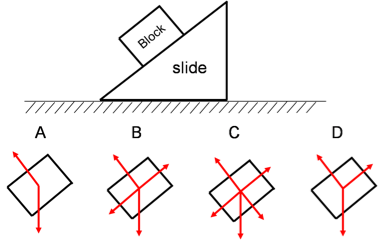
\includegraphics[scale=.4]{/Users/jgates/desktop/latex/pics/incline3.png}
%\end{floatingfigure}
 
{\bf \Large{\arabic{ProbNum}}} A fast RC car (speed: ${12~\tfrac{m}{s}}$ and a slower RC car (${8~\tfrac{m}{s}}$) are 40 meters apart. They then drive directly towards each other.  Some time after the cars have passed each other, the faster car is 15 meters away from the slower one.  

\bigskip

At this moment, how far has the slower one traveled from its starting position? 

%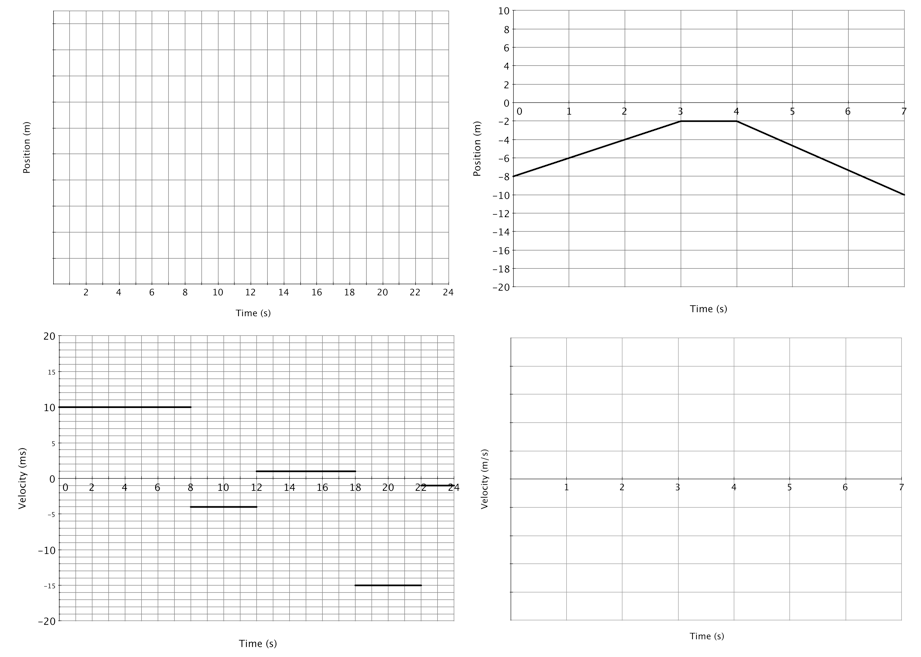
\includegraphics[scale=.57]{/Users/jgates/desktop/latex/pics/cvpmgraphs1.png}

\vfill

\newpage
